\documentclass[a4paper,11pt,titlepage]{article}
\parskip 3pt

%% %%%%%%%%%%%%%%%%%%%% BEGIN PACKAGES %%%%%%%%%%%%%%%%%%%%

%%\usepackage[top=1in, bottom=1in, left=1in, right=1in]{geometry}

\usepackage{fullpage}
\usepackage{url}
\usepackage{hyperref}
\hypersetup{pdfborder=0 0 0}

%% Images
\usepackage{graphicx}

%% Side-by-side images
\usepackage{subfig}

%% Drawing trees and other stuff
\usepackage{tikz}
\usetikzlibrary{trees,arrows}
\usepackage{amssymb}

%% Pseudocode
\usepackage[noend]{algorithmic}
\algsetup{indent=1.5em}

%% Linux Libertine
\usepackage[T1]{fontenc}
\usepackage{libertine}
\renewcommand*\oldstylenums[1]{{\fontfamily{fxlj}\selectfont #1}}

%% %%%%%%%%%%%%%%%%%%%% END PACKAGES %%%%%%%%%%%%%%%%%%%%


%% %%%%%%%%%%%%%%%%%%%% BEGIN COMMANDS %%%%%%%%%%%%%%%%%%%%

\let\stdhref\href
\renewcommand{\href}[2]{\stdhref{#1}{\texttt{#2}}}

\newcommand{\mailto}[1]{\href{mailto:#1}{#1}}

\let\stdsection\section         % because LaTeX cannot handle
                                % recursive commands
\renewcommand{\section}{\newpage\stdsection}

\let\tikzsquare\square
\renewcommand{\square}{\ensuremath\tikzsquare}

\newcommand{\code}[1]{\texttt{#1}}
\newcommand{\buzz}[1]{\emph{#1}}
\newcommand{\magic}[1]{\buzz{#1}}

%% %%%%%%%%%%%%%%%%%%%% END COMMANDS %%%%%%%%%%%%%%%%%%%%

%% %%%%%%%%%%%%%%%%%%%% BEGIN COLORS %%%%%%%%%%%%%%%%%%%%

\definecolor{cffffff}{RGB}{255,255,255}
\definecolor{c787aff}{RGB}{120,122,255}
\definecolor{cff7374}{RGB}{255,115,116}
\definecolor{c79ff79}{RGB}{121,255,121}
\definecolor{cff7374}{RGB}{255,115,116}
\definecolor{c7372ff}{RGB}{115,114,255}

%% %%%%%%%%%%%%%%%%%%%% END COLORS %%%%%%%%%%%%%%%%%%%%


%% Final Report -- due: 9th Jan 2012, at 11:00
%% Contents for Final Report: The project report should not be longer than 45 pages, and might be organized according to the following structure:

%% A. High Level, Nontechnical Description Why you should buy this product/listen to this presentation? What is the functionality of the product?
%% B. Short Technical Description
%% Short introduction into technologies used
%% Design of your software, possibly including a diagram of the major components of the project
%% Main achievements
%% C. Software Engineering Issues:
%% What technology was used and why; what other technology was considered but not used and why
%% Any technical challenges encountered and how addressed
%% Any risks anticipated, and how mitigated?
%% Any collaboration/coordination difficulties encountered and how addressed
%% Development and testing methods and/or tools used; comparison of plans with actual achievements
%% Estimates of length of code in each of the components, or any other comparable measure of the effort required.
%% Summary of each team member's contributions
%% D. Validation and Conclusions How did you validate your product? Was the project successful? What did you learn? What might you have done differently?
%% E. Bibliography
%% F. Appendix The appendix is optional, and does not count towards the 45 pages. It may contain thing like: User guide, installation instructions; more extensive design, testing, statistics etc.
%% Feel free to re-use material from the previous reports as you see fit, but make sure that the final report presents a coherent story. Ask advice from your supervisor. You might also draw inspiration from the instructions about writing up your individual project.

%% Bear in mind, that most of the project assessors will not have followed the project throughout and will only have a short time to listen to a presentation or see a demonstration. For this reason they will rely heavily on the report to judge the project.

%% The report should be submitted to SGO in form of a hard copy, as well as electronically through CATE.

\begin{document}
\title{\Huge Visigoth\\\Large Graph visualisations}
\author{
  Andreea-Ingrid Funie\\\mailto{aif109@doc.ic.ac.uk}\and
  Alexandru Scvor\c tov\\\mailto{as10109@doc.ic.ac.uk}\and
  Francesco Mazzoli\\\mailto{fm2209@doc.ic.ac.uk}\and
  Marc-David Haubenstock\\\mailto{mh808@doc.ic.ac.uk}\and
  Maximilian Staudt\\\mailto{ms9109@doc.ic.ac.uk}
}
\date{January 2012}
\maketitle

\begin{abstract}
%% FIXME: This needs more work.

Visigoth is a tool to generate, analyse and visualise Small World
Networks. These are particular kinds of graphs which \emph{look} like
natural networks and share many mathematical properties with them.
For instance, the friendship graphs and graphs of followers in modern
web-based social networks are Small World Networks.

Visigoth is an educational tool that allows users to explore Small
World Networks and hence can be used when introducing them. By
exploring these networks, users will have a firmer, more intuitive
grasp of the mathematical properties they exhibit.

The networks may be generated by one of several algorithms which
allows users to compare the varying quality of their output. The
generated networks form a smooth progression in the number of
exhibited desired properties from completely random graphs ---
generated by the Erdos-Renyi algorithm --- to Small World Networks ---
generated by the Preferential Attachment algorithm. Additionally,
Visigoth can connect to social networking platforms such as Twitter to
display real networks.
\end{abstract}

\tableofcontents




\section{Introduction}
%% This section corresponds to A in the requirements.

%% This section should contain most of the references to hamm10 and
%% oconn11.

Complex networks are ubiquitous in nature and society.

The structural and dynamical properties of complex networks are
non-trivial, and powerful computer architecture is needed for being
able to compute the required statistical analysis. As a result, it is
only in the last decade or so that we have been able to study the vast
data sets that describe real networks.\cite{oconn11}

The structural properties of real networks have been studied
extensively over the years. The main interest was focused on the fact
that many real networks share common characteristic properties. These
networks have low average length path, high clustering coefficient and
scale-free degree distribution. \cite{oconn11}

In order to be able to further understand the behaviour of real
networks, we simulate their dynamics on randomly generated networks.
For an accurate modelling of their behaviour we need to generate and
observe the results of algorithms which present the characteristic
structural properties of this kind of networks. \cite{oconn11}

\subsection{Realistic looking networks}
%% This subsection should *not* use the term ``Small World Networks''.
%% The point is to describe what properties we want.  The SWN
%% subsection below should be used in order to explain how they fit
%% the requirements.

%% FIXME: Define the qualities of the networks we want.  These
%% shouldn't be too mathy, just a layperson explanation (e.g. the
%% nodes shouldn't be too far apart, the number of neighbours should
%% fit a natural distribution).

The networks we are interested in are mathematical graphs in which
most nodes are not neighbors of one another, but they can be reached
from every other by a small number of steps. In the context of a
social network, this results in the \emph{``small world
  phenomenon''} \footnote{FIXME: citation needed} of strangers being
linked by a mutual acquaintance.

\subsubsection{Uses}

%% FIXME: Explain how networks with the above properties are useful.

Examples of real networks in the real-world are:

\emph{Social networks, neural networks, ecosystems, the World Wide
  Web, electrical power grids and protein networks} are all complex
networks that exhibit a range of understanding dynamic behaviour that
currently escape our understanding. \cite{oconn11}

Ideas from network science have been applied to the analysis of
metabolic and genetic regulatory networks, the design of robust and
scalable communication networks both wired and wireless, the
development of vaccination strategies for the control of disease, and
a broad range of other practical issues. \cite{complexNets}

\subsubsection{The maths}

%% FIXME: Give formal mathematical definitions for qualities.


\subsection{Small World Networks}

Small World Networks derive their denomination from the well-known
Small World Hypothesis\footnote{FIXME: citation needed}, which states
that any two persons are related through a chain of at most seven
friends\footnote{FIXME: citation needed}.

Indeed, Small World Networks are graphs resembling the connections
within human social networks, where nodes represent people, and edges
between nodes represent relations of some sort\footnote{FIXME:
  citation needed, probably one of the two main papers}.

For example, if someone were to draw every user\footnote{or at least a
  \emph{large} number of users} of a social network (e.g. Twitter) on
a canvas and then connect each pair of them if either is ``following''
the other or if they are ``friends'', the resulting graph is a Small
World Network. Over the course of time, several mathematical
algorithms that generate random Small World Networks have been
discovered. However, the resulting graphs have only lately begun to
resemble those that have grown naturally in the form of social
networks.

%% FIXME: Huh?  Are they really SWNs if they don't resemble the
%% natural graphs?  Not by our definition.  So, either the definition
%% is wrong, or the last two sentences need to be rewritten.

%% FIXME: Explain how SWNs exhibit *all* the properties we're
%% interested in.  Include some math.

\subsection{Introducing Visigoth}

Visigoth makes peeking into the current state-of-the-art of artificial
Small World Networks simple and fun. By integrating existing
generation algorithms and visualisations into a single, easy-to-use
interface, the user can make a head start into the small world of
Small World Networks and:
\begin{itemize}
  \item see how these algorithms have improved on each other over time
    generating increasingly better networks,
  \item see the effects of changing algorithm parameters on the
    resulting networks, and
  \item compare them to naturally grown networks.
\end{itemize}

\subsection{Customer requirements and iterative (re-)specification}

% What our customer wanted.
%
% What we suggested, and what he finally wanted.
% (E.g. once we suggested 3D he didn't want to let go of the idea)
%
% Finally, on overview of what we did, and what we added as a bonus.
% Possibly another subsection.

Our customer initially asked for a simple, easy-to-use, graphical
application that would allow him to compare various Small World
Network generation algorithms and parameters thereof, both visually
by looking at the graphs as well as numerically by calculating
several statistical properties of the graphs.
We suggested several additional features, such as a 3D view of the
graphs generated, real-world data fetching from social networks
(Twitter) and graph interaction. Following our customer's highly
positive reaction to our suggestions we then added them to our
product, creating a comprehensive base for analysing graphs that
may be re-used for other mathematical projects in the future.




%\section{In detail}
%% This section corresponds to B in the requirements

\section{Generating Small World Networks}
%% For all of the following, we should include a hand-drawn sketch
%% illustrating the graph generated by the algorithm and an exported
%% image of a large graph Visigoth generated.

\subsection{Erdos Renyi}

\subsection{Watts Strogatz}

\subsection{Bipartite Model}

\subsection{Preferential Attachment}

\subsection{Real Small World Networks}
Finally, as Visigoth is supposed to help in analysing Small World
Networks, it can also fetch real world data from `live' social
networks Twitter and identi.ca.




\section{Visigoth technologies}

\subsection{Qt}

The UI toolkit, standard library replacement, and application
framework Visigoth uses is Qt\footnote{\url{http://qt.nokia.com/}}.

Visigoth relies heavily on some of Qt's features:
\begin{description}
\item [gui] Qt is famous for providing a cross-platform, high-level,
  UI toolkit that automatically uses the native drawing systems on
  each host platform. All of Visigoth's user visible interface was
  built using this framework. A more detailed explanation is included
  in Section \ref{gui};
\item [meta-objects] Qt supplements the venerable C
  pre-processor\footnote{\url{http://gcc.gnu.org/onlinedocs/cpp/}}
  with its own \buzz{meta-object
    compiler} \footnote{\url{http://developer.qt.nokia.com/doc/qt-4.8/moc.html}}.
  This preprocessor augments normal C++ objects with modern features
  such as introspection and signals. We use introspection extensively
  in our tests; see Section \ref{tests}. We use signals to decouple
  objects, which leads to a cleaner design and has the side-effect of
  simplifying writing test cases (mock and stub objects are not
  necessary anymore); for details, see Section \ref{interaction};
\item [xml] Like most modern frameworks, Qt provides an \buzz{XML}
  parsing
  library\footnote{\url{http://developer.qt.nokia.com/doc/qt-4.8/qtxml.html}}.
  In addition to a standard \buzz{SAX} parser, it exposes an extremely
  clean \buzz{HTML DOM}-like interface for manipulating \buzz{XML}
  documents. We use it in order to parse results from queries to
  online sources such as \href{http://twitter.com}{Twitter} and
  \href{http://identi.ca}{Identi.ca};
\item [containers] Qt provides a fully-featured library of containers
  similar to Java
  \buzz{collections} \footnote{\url{http://docs.oracle.com/javase/1.5.0/docs/api/java/util/package-summary.html}}
  and significantly more complete than the standard or SGI
  \buzz{STL}\footnote{\url{http://www.sgi.com/tech/stl/}}. The
  availability of these meant that advanced data-structures were one
  less concern to worry about during development;
\item [concurrency] Qt also provides high-level
  threading\footnote{\url{http://developer.qt.nokia.com/doc/qt-4.8/threads.html}}
  and
  concurrency\footnote{\url{http://developer.qt.nokia.com/doc/qt-4.8/threads-qtconcurrent.html}}
  APIs. Our experiments showed that separating the CPU-intensive
  computations (e.g. generating new networks, calculating layout
  positions) onto a separate thread could speed up certain operations
  by as much as a factor of $6$. The concurrency API, which provides
  functional programming style parallelized primitives
  (e.g. \code{map}, \code{filter}) could further improve performance.
  This is an area where further work could be done in Visigoth.
\end{description}

\subsubsection{Plugins}

Qt has a healthy plugin ecosystems, with a myriad of libraries
available to plug into the main framework. We make use of two of
these, namely
\buzz{QCA} \footnote{\url{http://delta.affinix.com/qca/}} and
\buzz{QOAuth} \footnote{\url{https://github.com/ayoy/qoauth/wiki}}.

\begin{description}
\item [QCA] The \buzz{Qt Cryptographic Architecture} includes many
  security providers for Qt application. We used the \buzz{OpenSSL}
  provider when establishing TLS-secured channels to the online
  sources (e.g. \href{http://twitter.com}{Twitter});
\item [QOAuth] This library is an implementation of the \buzz{OAuth
  2.0}\footnote{\url{http://oauth.net/}} secure API authorization
  standard (\buzz{OAuth} is becoming the de-facto authorization
  mechanism on the web); again, this was required in order to
  authenticate with the online sources.
\end{description}

\subsubsection{Cross-platform}

Thanks to Qt's cross-platform nature, in general, and to
\buzz{qmake} \footnote{\url{http://developer.qt.nokia.com/doc/qt-4.8/qmake-manual.html}},
in particular, Visigoth works on Windows, OSX and Linux with a minimum
of fuss on the development side.

\begin{description}
\item [qmake] Qt's build system, \buzz{qmake}, takes a high level
  project description and outputs platform-specific build files
  (\buzz{Makefile}s on Linux, \buzz{XCode} projects on OSX and
  \buzz{Visual Studio} projects on Windows). It also simplifies
  finding external libraries (by using its own mechanism on Linux,
  \buzz{pkg-config} on OSX and the registry on Windows).
\end{description}

The only tweaks necessary for Visigoth to build on each of the above
platforms are a few defines to deal with the misplaced \buzz{OpenGL}
headers on OSX and few conditionals in the project description to
handle the library finding on Windows.

The following screenshots show Visigoth working on the three
platforms.
%% FIXME: add screenshots

\subsubsection{Rapid prototyping}

One of lesser known advantages to using Qt we discovered is rapid
prototyping. Point in case, the original prototype for Visigoth took
two days to write. It included roughly half of the customer's
\emph{must-have} features, was cross-platform and was visually
impressive.

\subsection{OpenGL}

After being left unsatisfied with the performance achieved with a
screen renderer using Qt graphics primitives, we looked for a `bare-metal'
graphics output solution in order to eliminate the graphics bottleneck.
Thanks to OpenGL\footnote{OpenGL documentation:
https://www.opengl.org/documentation/},
we can now draw even large graphs very quickly,
no matter whether in 2D or in 3D.

OpenGL itself is a graphics drawing interface commonly used to
leverage hardware acceleration for common operations, such as vector
transformations necessary to compute 3D graphics. Every modern
operating system uses it to animate its user interface smoothly,
and games and professional CAD (Computer Assisted Design) applications
have long used it for real-time 3D graphics interaction.

Not only are we leveraging this power to speed up our graph
visualiser, but this may also allow for ports to other
platforms in the future. Thanks to the Qt/OpenGL base, Visigoth
could theoretically be compiled for mobile phones and slates
with minimal porting effort.

OpenGL made several extensions possible, as outlined in the following
subsections.

\subsubsection{3D graphs and camera}
OpenGL provides only the very fundamental drawing primitives like
lines and points - however, it includes hardware acceleration for
vector transformation. This allows the implementation of a virtual
3D space through which a `camera' can move. As even this is actually
a composite functionality, we wrote a helper code library (glAncillary)
to provide us with easy camera transformation functions. They are
used whenever the user decides to move around the graph, i.e. to
pan or tilt.

\subsubsection{Selection}
The OpenGL interface also eases object selection: Since it is
responsible for the depth transformations when drawing the graphics,
it can also perform the inverse of these transformations from any
given point on the drawing surface, finding the original point
in space. In this case we check the position the mouse pointer is at
and find the object selected by the user. This is fundamental in
allowing us to move nodes around and selecting them for statistical
analysis.

\subsection{C++}

Visigoth, ignoring the XML files describing the interface, is entirely
written in \buzz{C++}. Initially, while being conscious of its disadvantages,
we made this decision for one reason: \buzz{Qt}. As described in the previous
paragraph, the library by TrollTech is so convenient that alone
justifies the use of C++ instead of another safer language.

All in all, we think it was the right decision. The appreciation of
C++ varies in our team, but looking back we are confident that C++ was
one of the best choices considering the nature of the application we
have been developing.

The main advantages were:

\begin{description}

\item [Availability of tools and library] As mentioned, \buzz{Qt} alone
  was a deal sealer, but the fact that we were able to access OpenGL
  `natively' (in a Qt widget) was also a big advantage. While interfaces
  to both libraries exist in other languages as well, we felt that
  sticking to Qt's `native' C++ environment would be the most stable
  solution and that the foreign language bindings would have degraded
  performance.

\item [Performance] We did not consider this factor at the beginning,
  but a few weeks into the project we started hitting various
  bottlenecks. We can only speculate about actual performance gains,
  but the fact that we were using
  C++ allowed us to fine-tune the application (specifically on the
  memory management side) in a way that we would not be able to do
  with managed languages. Furthermore, having an optimising compiler
  instead of an interpreter or JIT (as it would have been the case
  using a language like Python or Ruby) aided performance as well.

\item [Abstraction] The previous two points (especially the second)
  are partly shared by C++ with its predecessor, C. However, the
  possibility to structure our code into classes facilitates greatly
  structuring a medium sized application like Visigoth, especially
  considering that we had to coordinate five people working together.
  For example, there is a common \code{Algorithm} interface which all
  graph generation algorithms have to implement. They can then
  be plugged into the main widget at will: this kind of operation
  would have been much more laborious and less type-safe in C.

\end{description}

However, C++ also has its downsides:

\begin{description}

\item [Unmanaged memory] This is by far C++'s most ``dangerous''
  feature (or better, lack of feature). While enabling greater control
  and thus greater performance, it requires a much more attentive
  analysis of the code. This is in a way a good thing, since it forces
  the programmer to reason more about what the code is doing; but it
  also paves the way to a nasty class of bugs and memory leaks that
  more than once took hours (in one case days) to track down. This is
  a somewhat controversial subject in our team as well as the broader
  programming community and our opinions differ on how much better a
  garbage collected language would have been when considering the loss in
  performance. C++ also has the characteristic (required by its
  unmanaged nature) of allowing objects to be used in the heap through
  pointers and on the stack as values, which slows down compilation
  considerably - when changing a header file, all code that uses
  that object as a value has to be recompiled. Moreover, C++ allows two
  kinds of references: immutable references and C-style pointers, the
  former with
  a rather confusing syntax - references are indistinguishable from
  values when used. All these factors generate much confusion which is
  absent in most modern O-O languages.

\item [Language bloat] C++ is a very broad language with a number of
  esoteric language features. Notable examples are templates, operator
  overloading and ``friend'' attributes. Some of them are very
  useful and never harmful, e.g. the \code{const} keyword is a
  great mechanism to mark immutability at type level. However, some
  of them can and have been misused\footnote{For an hilarious example,
    see
    \url{http://weegen.home.xs4all.nl/eelis/analogliterals.xhtml}},
  and as a consequence ``when you're programming C++ no one can ever
  agree on which ten percent of the language is safe to use'' (Jamie
  Zawinski). This kind of ``programming language discipline'' is
  required when working on a C++ project and we had our fair share
  of arguments on which subset of the language is safe to use;
  nevertheless we think we have managed to keep the code clean to
  high standards in the C++ world.

\end{description}

This is of course only a very brief analysis of C++, but it does
highlight the points that we felt the most while developing Visigoth.




\section{Engineering Visigoth}
%% This section corresponds to C in the requirements

\subsection{GUI}
\label{gui}

\subsection{Classes}
%% This is an overview of the classes (including a class diagram).

\subsection{Object interaction}
\label{interaction}
%% This is an overview of the signals sent between objects (or of the
%% public interfaces they subscribe to).

\subsection{Graph drawing}

We looked into various graphics libraries which allow for
platform-independent drawing using primitives. Candidates were
\buzz{Cairo}\footnote{Cairo homepage: http://cairographics.org/},
\buzz{Qt} and \buzz{OpenGL}. The first two are the
most common 2D drawing libraries used in modern open-source
software; however, as they operate solely on the CPU, they proved
too slow for the large graphs we wished to visualise.

Therefore we decided to use \buzz{OpenGL} for drawing graphs on
the screen. Thanks to its hardware accelerated nature, we can now
(re-)draw thousands of nodes and edges often enough every second
to give the user the impression of a smooth interface when interacting
with the graph.

Implementing the camera handling, the node/edge drawing and the
interface allowing the user to `fly' through a 3D graph we also
developed a helper library, \code{glAncillary}. A significant portion
of our code can now be reused in similar projects using OpenGL,
and this is important since applications such as Visigoth require a
completely different type of graphics engine compared to the ones
commonly found e.g. in video games.


\subsection{Graph layout}
Laying out a graph is a tricky problem, mainly due to the fact that the
prime interest when engineering layouts is to please humans' taste
instead of some logical property. A wide array of such algorithms have
been proposed, and since drawing graphs is a central task in Visigoth,
we had to choose the one that fit best.

First we experimented with the existing solutions. One of the most
complete free graph-drawing algorithm is
OpenViz\footnote{\url{http://www.graphviz.org/}}, and it provides
various algorithms:

\begin{description}
\item [dot] A hierarchical layout, used for directed graphs. Our small
  world networks are not directed and it was clear from the beginning
  that they did not fit this model well.

\item [twopi, circo] Radial and circular layout, respectively. Again,
  unsuitable for the quasi-random networks that we use in Visigoth.

\item [neato] A spring model layout, which seemed to work reasonably
  well with random graphs.
\end{description}

The spring model seemed to be the best fit. This class of algorithm
work by treating edges like springs: in this way clusters of highly
connected nodes would be drawn together. To counter this force (that
would lead to nodes lumping together), nodes are treated as charged
particles of the same polarity, causing repulsion between every node
and the others.

When generating a graph, the nodes are first places at random
locations in the space. Then, we apply the algorithm repeatedly until
the forces are low enough that we can consider the graph to be stable.

Spring model algorithms are nice for two reasons:

\begin{itemize}
\item Good results: spring force algorithms produce pleasant graphs
  for almost all kind of networks. Some algorithms might produce
  better results for specific kinds of graph, but spring force
  algorithms are by far the more adaptive.

\item Ease of implementation: Our simple implementation of the
  algorithm take a little less then 50 lines of C++ code, and works
  well up to medium-sized graphs.

\item Real time drawing: force based algorithms can be used to show in
  real time the untangling of the graph, which is usually an
  interesting effect. It also permits interaction, for example in the
  form of node-dragging that changes the shape of the graph. We employ
  both techniques in Visigoth.
\end{itemize}

\subsubsection{FADE}

However, even a simple description of the algorithms reveals its high
cost. For each particle, we need to iterate through all the connected
nodes to calculate the spring forces, and more importantly through all
the particles of the graphs to calculate the repulsion forces. Thus,
the algorithm is \(O(n^2)\), where \(n\) is the number of nodes.

For this reason, our implementation works smoothly up to around a
\(1000\) nodes, but then performance degrades quickly, and the program
becomes unresponsive. Various solutions have been studied, most of
which rely on various approximations.

We chose to implement the \emph{FADE} algorithm \cite{fade}, which works by
recursively subdividing the graph space into sub-spaces, and then
treats sub-spaces as single particles when they are far enough. This
algorithm, while improving performance, is a lot more complex then the
naive one.

\begin{figure}
  \centering
  \subfloat[Graph view]{
    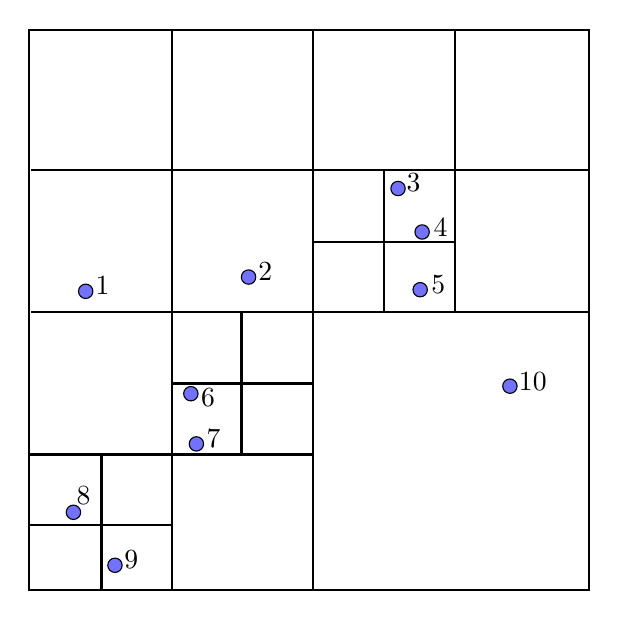
\begin{tikzpicture}[y=0.80pt, x=0.8pt,yscale=-0.5, xscale=0.5, inner sep=0pt, outer sep=0pt]
  \path[draw=black,line join=miter,line cap=butt,line width=0.800pt]
  (356.4286,94.5050) -- (356.4286,598.7908);
  \path[draw=black,line join=miter,line cap=butt,line width=0.800pt]
  (102.1429,348.7908) -- (605.7143,348.7908);
  \path[draw=black,line join=miter,line cap=butt,line width=0.800pt]
  (102.1429,220.2193) -- (607.1429,220.2193);
  \path[draw=black,line join=miter,line cap=butt,line width=0.800pt]
  (229.2857,93.0765) -- (229.2857,598.7908);
  \path[draw=black,line join=miter,line cap=butt,line width=0.800pt]
  (485.0000,93.7908) -- (485.0000,349.5050);
  \path[draw=black,line join=miter,line cap=butt,line width=0.800pt]
  (101.4286,477.3622) -- (356.4286,477.3622);
  \path[draw=black,line join=miter,line cap=butt,line width=0.800pt]
  (420.7143,220.2193) -- (420.7143,349.5050);
  \path[draw=black,line join=miter,line cap=butt,line width=0.800pt]
  (356.4286,285.2193) -- (485.0000,285.2193);
  \path[draw=black,line join=miter,line cap=butt,line width=0.800pt]
  (292.1429,348.0765) -- (292.1429,476.6479);
  \path[draw=black,line join=miter,line cap=butt,line width=0.800pt]
  (228.5714,413.0765) -- (357.1429,413.0765);
  \path[draw=black,line join=miter,line cap=butt,line width=0.800pt]
  (165.7143,477.3622) -- (165.7143,599.5050);
  \path[draw=black,line join=miter,line cap=butt,line width=0.800pt]
  (100.7143,540.9336) -- (229.2857,540.9336);
  \path[cm={{0.86607143,0.0,0.0,0.86607143,(-133.53636,-75.700851)}},draw=black,fill=c7372ff]
  (506.4286,453.4336)arc(0.000:180.000:7.500)arc(-180.000:0.000:7.500) -- cycle;
  \path[cm={{0.86607143,0.0,0.0,0.86607143,(-280.6792,-62.843726)}},draw=black,fill=c7372ff]
  (506.4286,453.4336)arc(0.000:180.000:7.500)arc(-180.000:0.000:7.500) -- cycle;
  \path[cm={{0.86607143,0.0,0.0,0.86607143,(-185.6792,29.656274)}},draw=black,fill=c7372ff]
  (506.4286,453.4336)arc(0.000:180.000:7.500)arc(-180.000:0.000:7.500) -- cycle;
  \path[cm={{0.86607143,0.0,0.0,0.86607143,(-180.6792,75.013418)}},draw=black,fill=c7372ff]
  (506.4286,453.4336)arc(0.000:180.000:7.500)arc(-180.000:0.000:7.500) -- cycle;
  \path[cm={{0.86607143,0.0,0.0,0.86607143,(-291.75062,136.79913)}},draw=black,fill=c7372ff]
  (506.4286,453.4336)arc(0.000:180.000:7.500)arc(-180.000:0.000:7.500) -- cycle;
  \path[cm={{0.86607143,0.0,0.0,0.86607143,(-254.25063,184.65628)}},draw=black,fill=c7372ff]
  (506.4286,453.4336)arc(0.000:180.000:7.500)arc(-180.000:0.000:7.500) -- cycle;
  \path[cm={{0.86607143,0.0,0.0,0.86607143,(102.53509,22.87056)}},draw=black,fill=c7372ff]
  (506.4286,453.4336)arc(0.000:180.000:7.500)arc(-180.000:0.000:7.500) -- cycle;
  \path[cm={{0.86607143,0.0,0.0,0.86607143,(21.463659,-64.272297)}},draw=black,fill=c7372ff]
  (506.4286,453.4336)arc(0.000:180.000:7.500)arc(-180.000:0.000:7.500) -- cycle;
  \path[cm={{0.86607143,0.0,0.0,0.86607143,(23.249374,-116.41515)}},draw=black,fill=c7372ff]
  (506.4286,453.4336)arc(0.000:180.000:7.500)arc(-180.000:0.000:7.500) -- cycle;
  \path[cm={{0.86607143,0.0,0.0,0.86607143,(1.4636592,-155.70087)}},draw=black,fill=c7372ff]
  (506.4286,453.4336)arc(0.000:180.000:7.500)arc(-180.000:0.000:7.500) -- cycle;
  \path[fill=black] (160.31509,332.78058) node[above right] (text6462) {1};
  \path[fill=black] (307.43341,319.70856) node[above right] (text6462-4) {2};
  \path[fill=black] (441.40405,239.94313) node[above right] (text6462-9) {3};
  \path[fill=black] (465.61832,280.30029) node[above right] (text6462-98) {4};
  \path[fill=black] (463.73944,332.14725) node[above right] (text6462-5) {5};
  \path[fill=black] (255.68974,433.98373) node[above right] (text6462-0) {6};
  \path[fill=black] (260.68976,470.65741) node[above right] (text6462-7) {7};
  \path[fill=black] (143.21951,522.34161) node[above right] (text6462-3) {8};
  \path[fill=black] (186.40405,580.65741) node[above right] (text6462-43) {9};
  \path[fill=black] (542.83264,419.586) node[above right] (text6462-02) {10};
  \path[draw=black,line join=miter,line cap=butt,line width=0.800pt]
  (606.0915,92.7173) -- (606.0915,599.8138) -- (100.0051,599.8138) --
  (100.0051,92.7173);
  \path[draw=black,line join=miter,line cap=butt,line width=0.800pt]
  (100.0051,93.7274) -- (605.0814,93.7274);
\end{tikzpicture}

  }
  \hspace{10pt}
  \subfloat[Tree representation]{
    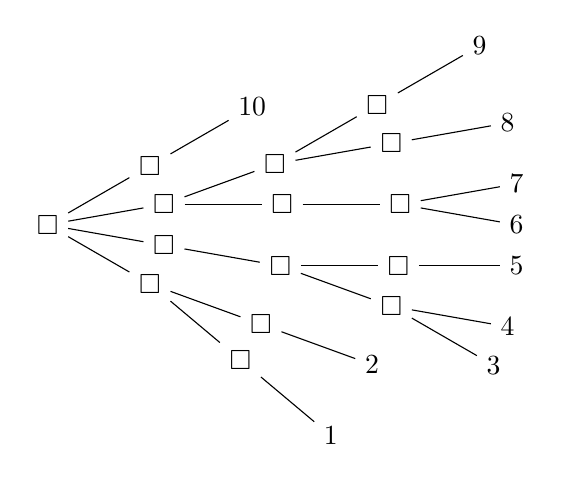
\begin{tikzpicture}[grow cyclic]
  \node {\square}
  child {
    node {\square}
    child {
      node {\square}
      child {node {1}}
    }
    child {
      node {\square}
      child {node {2}}
    }
  }
  child {
    node {\square}
    child {
      node {\square}
      child {
        node {\square}
        child { node{3} }
        child { node{4} }
      }
      child {
        node {\square}
        child {node{5}}
      }
    }
  }
  child {
    node {\square}
    child {
      node {\square}
      child {
        node {\square}
        child {node{6}}
        child {node{7}}
      }
    }
    child {
      node {\square}
      child {
        node {\square}
        child {node{8}}
      }
      child {
        node {\square}
        child {node{9}}
      }
    }
  }
  child {
    node {\square}
    child { node {10} }
  }
  ;
\end{tikzpicture}

  }
  \caption{The QuadTree for a sample graph, empty branches omitted}
  \label{fig:quadtree}
\end{figure}

The first step is to build a data structure representing the recursive
subdivision. This kind of data structure is called a \emph{TreeCode},
which recursively subdivides the space until only one node remains in
the current space, or a maximum depth/minimum space size size is
hit. The space decomposition can be irregular (e.g. \emph{Voronoi}
spaces) or regular. In the latter case, the space is recursively
subdivided in squares. We chose to use a regular, 4-way space
decomposition, mainly due to its simplicity. This kind of structure is
called \emph{QuadTree}. Figure \ref{fig:quadtree} shows a sample
QuadTree for a Visigoth graph. In the QuadTree, each sub-quadrant
preserved the weighted centre of gravity relative to the contained
nodes.

Building the tree is the difficult part of the algorithm and can be
done in linear time. Once that is done, to calculate the non-edge
forces for a given node the algorithm proceeds as indicated in figure
\ref{proc:FADE}.

\begin{figure}[ht]
  \begin{minipage}[b]{0.5\linewidth}
    \begin{algorithmic}
  \REQUIRE \(0 < \theta < 1\)
  \REQUIRE \(\beta > 1\)
  \REQUIRE \(\vec{n} \neq \vec{q}\)
\end{algorithmic}
force\((n, q)\):
\begin{algorithmic}
  \STATE \(\vec{d} \gets \vec{n} - \vec{q}\)
  \IF { \(q\) is terminal \OR \(\frac{\vec{d}}{\textrm{width}(q)} < \theta\) }
  \STATE \(\vec{v} \gets \vec{d} \cdot \frac{\beta}{|{\vec{d}}|^2}\)
  \STATE \(\vec{v} \gets \vec{v} \cdot \textrm{mass}(q)\)
  \RETURN \(\vec{v} \cdot \frac{\beta}{|{\vec{d}}|^2}\)
  \ELSE
  \STATE \(\vec{v} \gets 0\)
  \FOR {\(q'\) in children\((q)\)}
  \STATE \(\vec{v} \gets \vec{v} + \textrm{force}(n, q')\)
  \ENDFOR
  \RETURN \(\vec{v}\)
  \ENDIF
\end{algorithmic}

    \caption{This procedure calculates the non-edge force of a given
      node \(n\), given the QuadTree \(q\). \(\vec{n}\) and
      \(\vec{q}\) indicate the vectors corresponding to the respective
      centers of gravity. \(\beta\) is an empirically determined
      parameter used to regulate the amount of force - \(75\) has
      worked well for us. \(\theta\) is central to the FADE algorithm
      and determines the amount of approximation. If \(\geq 1\) the
      algorithm is unstable, we used values between \(0.5\) and
      \(0.8\). See figure \ref{fig:theta} for a visual
      explanation. The mass of a quadrant is simply the number of
      nodes residing in it. }
    \label{proc:FADE}
  \end{minipage}
  \hspace{10pt}
  \begin{minipage}[b]{0.5\linewidth}
    \centering
    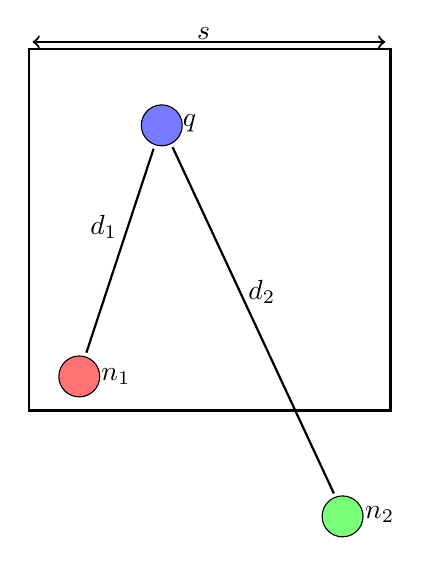
\begin{tikzpicture}[y=0.80pt, x=0.8pt,yscale=-1, inner sep=0pt, outer sep=0pt]
  \path[draw=black,fill=cffffff,line join=miter,line cap=butt,fill
    opacity=0.000,even odd rule,line width=0.803pt,rounded corners=0.0000cm]
  (140.4134,176.5621) rectangle (303.7579,339.9066);
  \path[cm={{0.79503474,0.0,0.0,0.79503474,(-296.23722,-12.403676)}},draw=black,fill=c787aff]
  (636.3961,281.1107)arc(0.000:180.000:11.617)arc(-180.000:0.000:11.617) --
  cycle;
  \path[cm={{0.79503474,0.0,0.0,0.79503474,(-333.50701,101.01225)}},draw=black,fill=cff7374]
  (636.3961,281.1107)arc(0.000:180.000:11.617)arc(-180.000:0.000:11.617) --
  cycle;
  \path[cm={{0.79503474,0.0,0.0,0.79503474,(-214.57843,164.22654)}},draw=black,fill=c79ff79]
  (636.3961,281.1107)arc(0.000:180.000:11.617)arc(-180.000:0.000:11.617) --
  cycle;
  \path[draw=black,line join=miter,line cap=butt,line width=0.800pt]
  (166.4286,313.7908) -- (196.7857,221.6479);
  \path[draw=black,line join=miter,line cap=butt,line width=0.800pt]
  (205.3571,220.9336) -- (278.2143,377.3622);
  \path[fill=black] (168.21428,262.36218) node[above right] (text5235) {\(d_1\)};
  \path[fill=black] (239.64287,291.64789) node[above right] (text5239) {\(d_2\)};
  \path[fill=black] (216.42857,172.36218) node[above right] (text5243) {\(s\)};
  \path (142.5000,173.7908) -- (300.0000,173.7908);
  \path[draw=black,line join=miter,line cap=butt,line width=0.800pt, <->]
  (142.1429,173.4336) -- (301.4286,173.4336);
  \path[fill=black] (210,214.1479) node[above right] (text5479) {\(q\)};
  \path[fill=black] (173.21429,328.07648) node[above right] (text5483) {\(n_1\)};
  \path[fill=black] (292.34625,390.3728) node[above right] (text5483-5) {\(n_2\)};
\end{tikzpicture}

    \caption{In this case, \(n_1\) and \(n_2\) are nodes and \(q\) is
      a quadrant with edge length \(s\). When calculating the non-edge
      force between \(n_1\) and \(q\), where \(s\) is the quadrant
      will be judged to be too close to approximate, since
      \(\frac{s}{d_1} > 1\), while \(n_2\) might be judged far enough,
      depending on \(\theta\).}
    \label{fig:theta}
  \end{minipage}
\end{figure}

Once implemented, the FADE algorithm lead to great speedups while
preserving good node placements. While drawing \(1000\) nodes is
already difficult with the simple algorithm, FADE can easily handle
\(10000\) nodes, after which other performance limits are hit (the
graph generation time and the OpenGL drawing).

After we implemented the 3D view we had to write an extension to FADE to support
3D, which proved to be straight forward. Now we have a 3-dimensional space,
which is recursively divided into $8$ cubes.




\section{Looking back}
%% This section corresponds to 'Conclusions' in part D of the requirements

\subsection{Validation}
%% The client is a happy puppy

\subsection{Functional testing}
\label{tests}

\subsection{Lessons learned}

\addcontentsline{toc}{section}{References}
\begin{thebibliography}{9}

\bibitem{hamm10}
  David A. Hammond,
  \emph{Altruism in Small World Models}.
  Imperial College London,
  2010.

\bibitem{oconn11}
  Luke M. O'Connor,
  \emph{Algorithms for Constructing Realistic Networks}.
  Imperial College London,
  2011.

\bibitem{fade}
  Aaron Quigley and Peter Eades,
  \emph{FADE: Graph drawing, clustering and visual abstraction}.
  Department of Computer Science and Software Engineering,
  Univ. of  Newcastle, Australia, 2000.

\bibitem{complexNets}
  \url{http://en.wikipedia.org/wiki/Complex_network}

\end{thebibliography}

\end{document}
